\documentclass[12pt,letterpaper]{article}
\usepackage{graphicx,textcomp}
\usepackage{natbib}
\usepackage{setspace}
\usepackage{fullpage}
\usepackage{color}
\usepackage[reqno]{amsmath}
\usepackage{amsthm}
\usepackage{fancyvrb}
\usepackage{amssymb,enumerate}
\usepackage[all]{xy}
\usepackage{endnotes}
\usepackage{lscape}
\newtheorem{com}{Comment}
\usepackage{float}
\usepackage{hyperref}
\newtheorem{lem} {Lemma}
\newtheorem{prop}{Proposition}
\newtheorem{thm}{Theorem}
\newtheorem{defn}{Definition}
\newtheorem{cor}{Corollary}
\newtheorem{obs}{Observation}
\usepackage[compact]{titlesec}
\usepackage{dcolumn}
\usepackage{tikz}
\usetikzlibrary{arrows}
\usepackage{multirow}
\usepackage{xcolor}
\newcolumntype{.}{D{.}{.}{-1}}
\newcolumntype{d}[1]{D{.}{.}{#1}}
\definecolor{light-gray}{gray}{0.65}
\usepackage{url}
\usepackage{listings}
\usepackage{color}

\definecolor{codegreen}{rgb}{0,0.6,0}
\definecolor{codegray}{rgb}{0.5,0.5,0.5}
\definecolor{codepurple}{rgb}{0.58,0,0.82}
\definecolor{backcolour}{rgb}{0.95,0.95,0.92}

\lstdefinestyle{mystyle}{
	backgroundcolor=\color{backcolour},   
	commentstyle=\color{codegreen},
	keywordstyle=\color{magenta},
	numberstyle=\tiny\color{codegray},
	stringstyle=\color{codepurple},
	basicstyle=\footnotesize,
	breakatwhitespace=false,         
	breaklines=true,                 
	captionpos=b,                    
	keepspaces=true,                 
	numbers=left,                    
	numbersep=5pt,                  
	showspaces=false,                
	showstringspaces=false,
	showtabs=false,                  
	tabsize=2
}
\lstset{style=mystyle}
\newcommand{\Sref}[1]{Section~\ref{#1}}
\newtheorem{hyp}{Hypothesis}

\title{Problem Set 1}
\date{Due: October 8, 2026}
\author{Applied Stats/Quant Methods 1}
\author{Owen Stidman}

\begin{document}
	\maketitle
	
	\section*{Instructions}
	\begin{itemize}
		\item Please show your work! You may lose points by simply writing in the answer. If the problem requires you to execute commands in \texttt{R}, please include the code you used to get your answers. Please also include the \texttt{.R} file that contains your code. If you are not sure if work needs to be shown for a particular problem, please ask.
		\item Your homework should be submitted electronically on GitHub.
		\item This problem set is due before 23:59 on Thursday October 8, 2026. No late assignments will be accepted.
	\end{itemize}
	
	\vspace{1cm}
	
	\textbf{\textit{*** In the interest of academic integrity: I relied heavily on StackOverflow, Google, and the Code Camp materials for assistance with the programming in this assignment. I did not use any AI. As I oppose AI in general, I will not use any AI during this Master's programme unless explicity instructed to do so by a professor or teaching assistant. }}
	
	\section*{Question 1: Education}
	
	A school counselor was curious about the average of IQ of the students in her school and took a random sample of 25 students' IQ scores. The following is the data set:\\
	\vspace{.5cm}
	
	\lstinputlisting[language=R, firstline=51, lastline=51]{PS01_answers_OS.R}  
	
	
	\vspace{1cm}
	
	\begin{enumerate}
		\item Find a 90\% confidence interval for the average student IQ in the school (As a hint, you first need the mean and SD to create a CI):\\
		
		First, I calculate the mean and standard deviation to construct the confidence interval and assigning to objects with descriptive variable names:
		\lstinputlisting[language=R, firstline=55, lastline=56]{PS01_answers_OS.R}
		
		Next, I return the values of the sample mean IQ and sample standard deviation:
		\lstinputlisting[language=R, firstline=59, lastline=60]{PS01_answers_OS.R}

		
		The sample size \textit{n} = 25; therefore, the degrees of freedom \textit{df} = \textit{n}-1 = 24. The formula for a confidence interval for a mean is $\bar{y}$ ± \textit{t(s / $\sqrt{n}$)}, where $\bar{y}$ is the sample mean, \textit{t} is the critical value from the  \textit{t}-distribution, \textit{s} is the sample standard deviation, and \textit{n} is the sample size. The value s / $\sqrt{n}$ is the standard error.
		
		As we know $\bar{y}$ (98.44 mean IQ, calculated previously), \textit{s} (13.09287, calculated previously), and \textit{n} (given), the only remaining unknown value is the critical value from the \textit{t}-distribution. 
		
		Using Table B (\textit{t}-distribution critical values) from the Agresti and Finlay 2009 textbook, we see that the critical value for a 90 percent confidence interval with degrees of freedom \textit{df} = 24 is \textit{t} = 1.711.
		
		Therefore, $\bar{y}$ ± t(s / $\sqrt{n}$) = 98.44 ± 1.711(13.09287/$\sqrt{25}$)
		= 98.44 ± 1.711(13.09287/5).
		
		I calculate the lower and upper values of the 90 percent confidence interval and assign them to objects: 
		\lstinputlisting[language=R, firstline=82, lastline=83]{PS01_answers_OS.R}
		
		I return the the lower and upper values of the interval:
		\lstinputlisting[language=R, firstline=86, lastline=87]{PS01_answers_OS.R}
		
		This returns 93.95962 and 102.9204, respectively.
		
		\textbf{The 90 percent confidence interval for the mean IQ score is [93.95962, 102.9204].} If this study were performed 100 times, this interval would be expected to contain the true population mean IQ score 90 percent of the times. 
		
		\item Next, the school counselor was curious  whether  the average student IQ in her school is higher than the average IQ score (100) among all the schools in the country.\\ 
		
		\noindent Using the same sample, conduct the appropriate hypothesis test with $\alpha=0.05$. 
		\vspace{.5cm}
		
		\textit{Although the counselor is wondering whether the mean IQ of students at the school is "higher than" (rather than "different than") the nationwide average IQ of 100, the sample mean of 98.44 is \textit{lower} than 100. This suggests that, in spite of the counselor's "higher than" framing, a two-sided significance test, rather than a one- sided test, may be more appropriate.}
		
		\textbf{1. ASSUMPTIONS: }
		
		We can safely assume that the data in question is quantitative, as IQ is always measured numerically. 
		
		We can reasonably assume the sample was randomly selected, as the assignment states that the counselor "took a random sample." We cannot, however, assume that the sample size \textit{n} was greater than or equal to 30, as it is explicitly stated that \textit{n = 25.} We will therefore use a t-score, rather than a z-score, in conducting our hypothesis test. 
		
		That said, we can reasonably assume the variable in question (IQ) has a normal population distribution, as "Most people score near the average range, which is designed to fit into a normal distribution curve" (Kendra Cherry, MSEd).
		
		\textbf{2. HYPOTHESES: }
		
		Let \textit{meanIQ} denote the mean IQ.
		
		\textit{$H_0$: meanIQ} = 100
		
		\textit{$H_a$: meanIQ} $\neq$ 100
		
		\textbf{3. TEST STATISTIC: }
		
		The \textit{n} = 25 observations are summarized by a sample mean IQ of 98.44 and a sample standard deviation of 13.09287, both calculated previously.
		
		The degrees of freedom \textit{df = n} - 1 = 24. 
		
		The estimated standard error is \textit{se = s / $\sqrt{n}$} = 13.09287 / 5.
		
		\lstinputlisting[language=R, firstline=126, lastline=126]{PS01_answers_OS.R}
		
		This computes to 2.618574.
		
		The value of the test statistic is the difference between the observed sample mean (98.44) and the population mean (100) divided by the standard error (2.618574).
		
		\lstinputlisting[language=R, firstline=132, lastline=133]{PS01_answers_OS.R}
		
		This computes to -0.5957439.
		
		In other words, the sample mean falls 0.5957439 estimated standard errors below the null hypothesis value of the mean. 
		
		\textbf{4. P-VALUE:}
		
		The P-value is the two-tail probability,  presuming $H_0$ is true, that \textit{t} would exceed 0.5957439 in absolute value.  From the \textit{t}-distribution with \textit{df} = 24, this two-tail probability is:
		
		\lstinputlisting[language=R, firstline=145, lastline=146]{PS01_answers_OS.R}
		
		Using the "pt" command in R \textbf{\textit{(found online through a Google search, no AI  used)}}, this computes to \textit{P} = 0.5569233.
		
		With our $\alpha$-level of 0.05, \textit{P} $>$ $\alpha$. 
		
		\textbf{5. CONCLUSION}
		
		\textbf{We fail to reject the null hypothesis at the \textit{alpha} = 0.05 significance level. The counselor's findings are not statistically significant. }
	\end{enumerate}
	
	\newpage
	
	\section*{Question 2: Political Economy}
	
	\noindent Researchers are curious about what affects the amount of money communities spend on addressing homelessness. The following variables constitute our data set about social welfare expenditures in the USA. \\
	\vspace{.5cm}
	
	
	\begin{tabular}{r|l}
		\texttt{State} &\emph{50 states in US} \\
		\texttt{Y} & \emph{per capita expenditure on shelters/housing assistance in state}\\
		\texttt{X1} &\emph{per capita personal income in state} \\
		\texttt{X2} &  \emph{Number of residents per 100,000 that are "financially insecure" in state}\\
		\texttt{X3} &  \emph{Number of people per thousand residing in urban areas in state} \\
		\texttt{Region} &  \emph{1=Northeast, 2= North Central, 3= South, 4=West} \\
	\end{tabular}
	
	\vspace{.5cm}
	\noindent Explore the \texttt{expenditure} data set and import data into \texttt{R}.
	\vspace{.5cm}
	
	I import the data into R and save a copy using the following commands:
	\lstinputlisting[language=R, firstline=160, lastline=161]{PS01_answers_OS.R}
	
	I generate some preliminary exploratory statistics using the following commands:
	\lstinputlisting[language=R, firstline=165, lastline=168]{PS01_answers_OS.R}
	
	The "str" command outputs the internal structure of the data frame, which in this case includes 50 observations -- i.e. 50 states -- of the six variables listed above. 
	
		\vspace{.5cm}
	The "summary" command produces the following output: 
	
	\begin{verbatim}
		 STATE          Y                X1             X2       
		Length   :50   Min.   : 42.00   Min.   :1053   Min.   :111.0  
		N.unique :50   1st Qu.: 67.25   1st Qu.:1698   1st Qu.:187.2  
		N.blank  : 0   Median : 79.00   Median :1897   Median :241.5  
		Min.nchar: 2   Mean   : 79.54   Mean   :1912   Mean   :281.8  
		Max.nchar: 2   3rd Qu.: 90.00   3rd Qu.:2096   3rd Qu.:391.8  
		Max.   :129.00   Max.   :2817   Max.   :531.0  
		X3            Region    
		Min.   :326.0   Min.   :1.00  
		1st Qu.:426.2   1st Qu.:2.00  
		Median :568.0   Median :3.00  
		Mean   :561.7   Mean   :2.66  
		3rd Qu.:661.2   3rd Qu.:3.75  
		Max.   :899.0   Max.   :4.00  
	\end{verbatim}
	
		\vspace{.5cm}
	
	The "head" command produces the following output:
	
	\begin{verbatim}
		 STATE  Y   X1  X2  X3 Region
		1    ME 61 1704 388 399      1
		2    NH 68 1885 272 598      1
		3    VT 72 1745 397 370      1
		4    MA 72 2394 458 868      1
		5    RI 62 1966 157 899      1
		6    CT 91 2817 162 690      1
	\end{verbatim}
	
	\vspace{.5cm}

	The "glimpse" command produces the following output:
	
\begin{verbatim}
	Rows: 50
	Columns: 6
	$ STATE  <chr> "ME", "NH", "VT", "MA", "RI", "CT", "NY", "NJ", "PA"…
	$ Y      <int> 61, 68, 72, 72, 62, 91, 120, 99, 70, 82, 84, 84, 104…
	$ X1     <int> 1704, 1885, 1745, 2394, 1966, 2817, 2685, 2521, 2127…
	$ X2     <int> 388, 272, 397, 458, 157, 162, 494, 153, 152, 187, 19…
	$ X3     <int> 399, 598, 370, 868, 899, 690, 728, 826, 656, 674, 56…
	$ Region <int> 1, 1, 1, 1, 1, 1, 1, 1, 1, 2, 2, 2, 2, 2, 2, 2, 2, 2…
\end{verbatim}
	
	
	\lstinputlisting[language=R, firstline=42, lastline=42]{PS01_answers_OS.R}  
	\vspace{.5cm}
	\begin{itemize}
		
		\item
		Please plot the relationships among \emph{Y}, \emph{X1}, \emph{X2}, and \emph{X3}? What are the correlations among them (you just need to describe the graph and the relationships among them)?
		
		\textbf{1. Relationship between Y (housing expenditure) and X1 (income)}
		
		I create a simple linear regression model and calculate the slope, intercept, and correlation (R-squared):
		\lstinputlisting[language=R, firstline=174, lastline=176]{PS01_answers_OS.R}
		
		I generate the below scatterplot using the following code:
		\lstinputlisting[language=R, firstline=182, lastline=191]{PS01_answers_OS.R}
		
		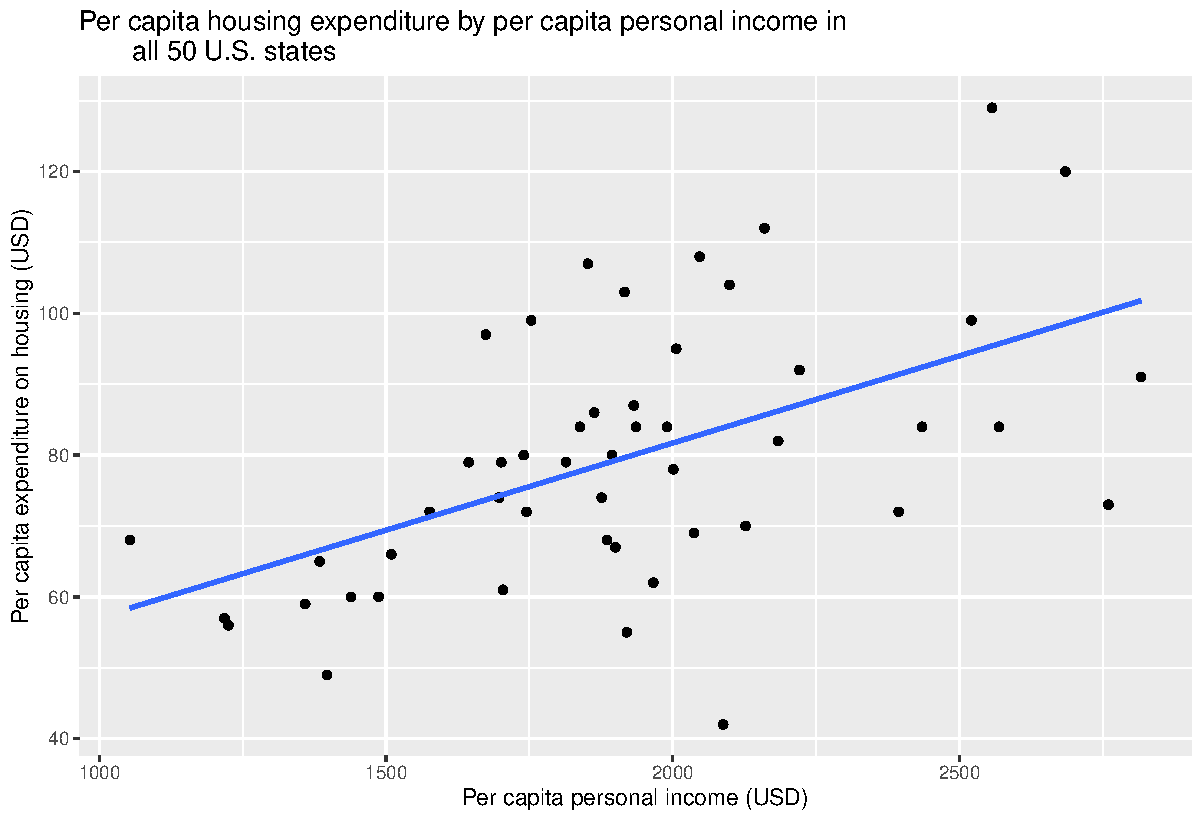
\includegraphics[scale=0.7]{housingByIncomePlot}\\
		
		This scatterplot shows a weak, positive association between per capita personal income and per capita expenditure on housing assistance. There do not appear to be any outliers in the data. The multiple R-squared value is  0.2827; the adjusted R-squared value is  0.2678. The linear regression model is \textit{per capita housing expenditure = 0.02458(per capita personal income) + 32.546152 + $\epsilon$}.
		
		\textbf{2. Relationship between Y (housing expenditure) and X2 (financial insecurity)}
		
		I create a simple linear regression model and calculate the slope, intercept, and correlation (R-squared):
		\lstinputlisting[language=R, firstline=197, lastline=199]{PS01_answers_OS.R}
		
		I generate the below scatterplot using the following code:
		\lstinputlisting[language=R, firstline=205, lastline=216]{PS01_answers_OS.R}
		
		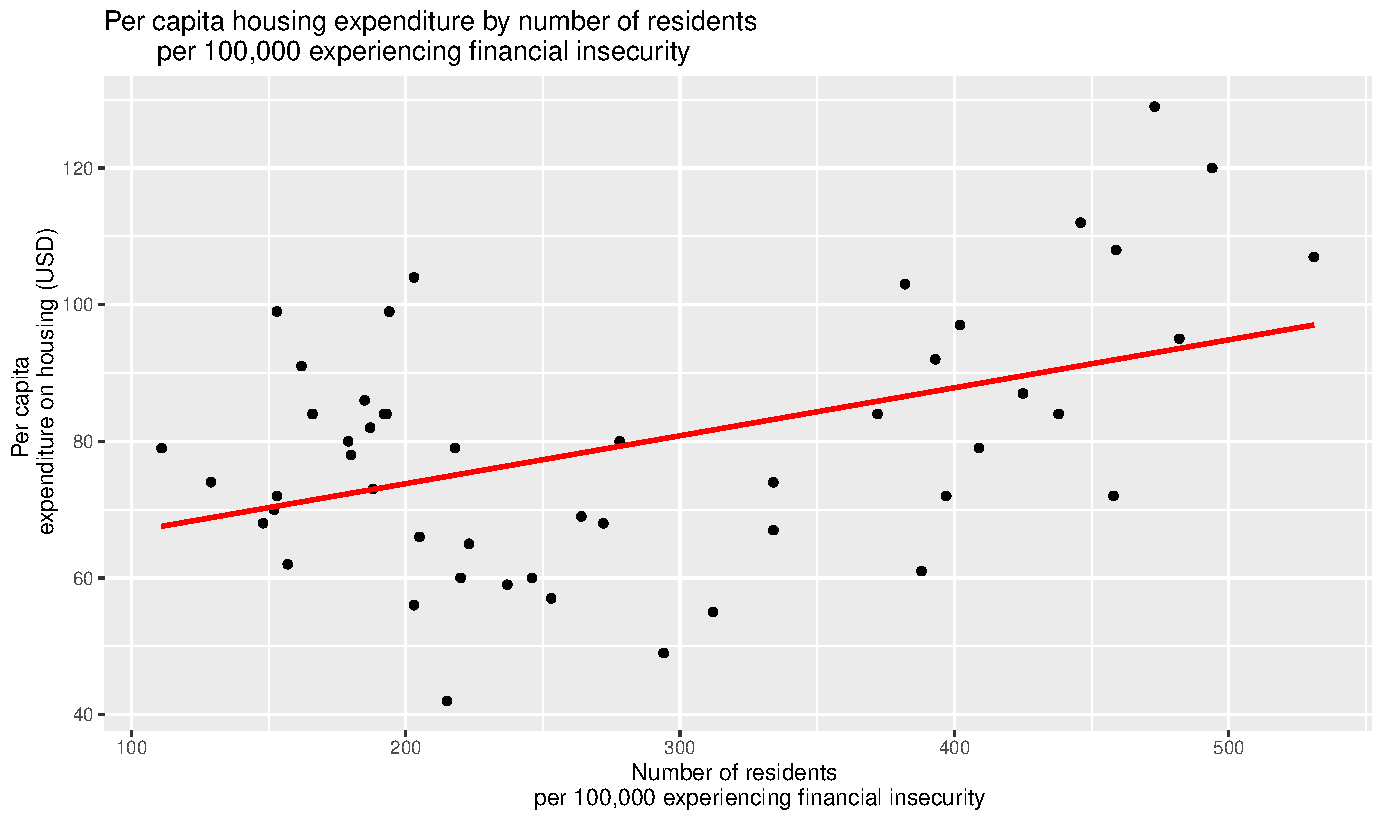
\includegraphics[scale=0.7]{housingByFinancialInsecurityPlot}
		
		This scatterplot shows a weak, positive association between the number of residents per 100,000 experiencing financial insecurity and per capita expenditure on housing assistance. There do not appear to be any outliers in the data. The multiple R-squared value is  0.201; the adjusted R-squared value is  0.1843. The linear regression model is \textit{per capita housing expenditure = 0.07019(residents per 100k experiencing financial insecurity) + 59.76104 + $\epsilon$}.
		
		\textbf{3. Relationship between Y (housing expenditure) and X3 (urban population)}
		
		I create a simple linear regression model and calculate the slope, intercept, and correlation (R-squared):
		\lstinputlisting[language=R, firstline=222, lastline=224]{PS01_answers_OS.R}
		
		I generate the below scatterplot using the following code:
		\lstinputlisting[language=R, firstline=230, lastline=241]{PS01_answers_OS.R}
		
		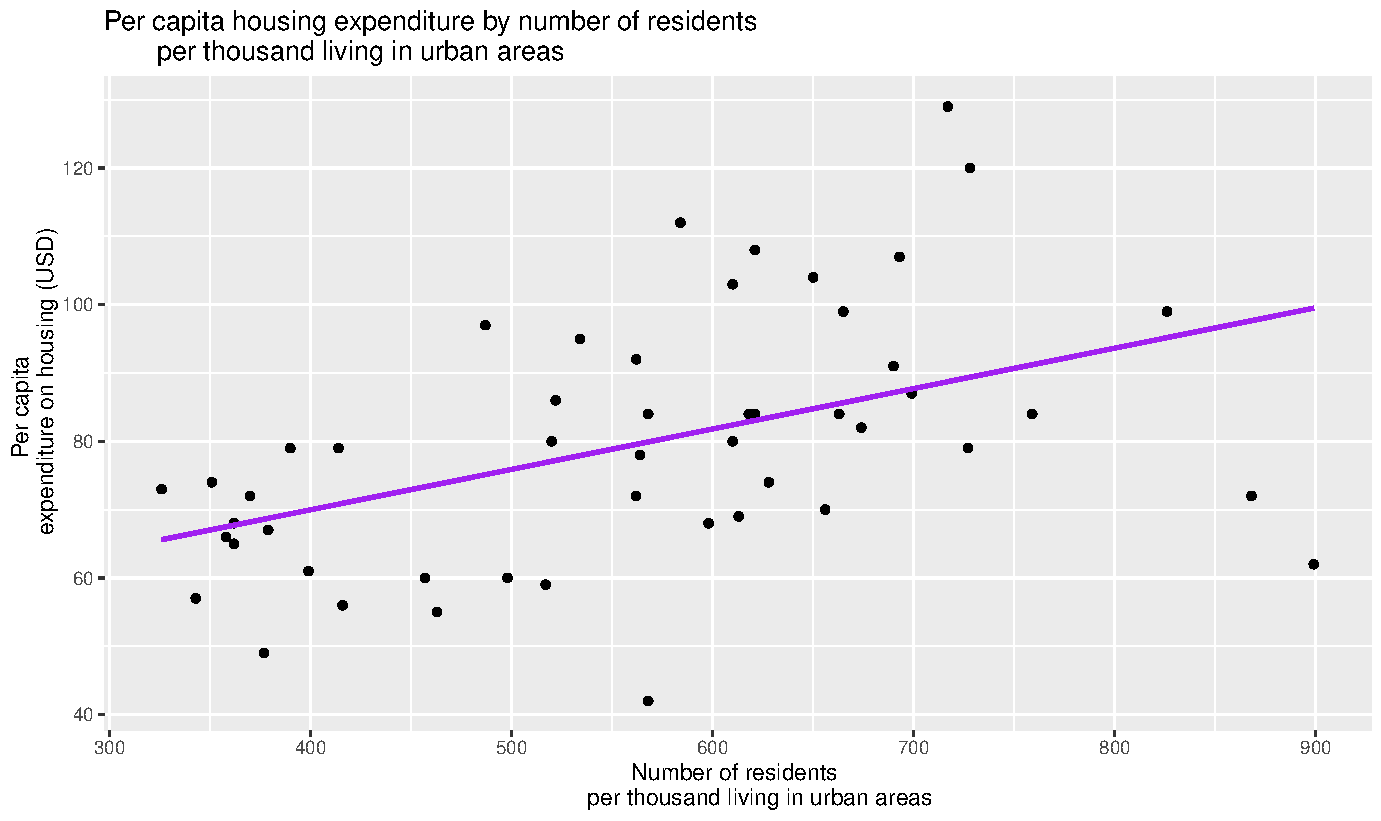
\includegraphics[scale=0.7]{housingByUrbanPopulationPlot}
		
		This scatterplot shows a weak, positive association between the number of residents per 100,000 living in urban areas and per capita expenditure on housing assistance. The two observations representing the states with the most residents in urban areas and reltively low housing expenditures may be outliers. The multiple R-squared valus is  0.215; the	adjusted R-squared value is  0.1986. The linear regression model is \textit{per capita housing expenditure = 0.05917(residents per 100k in urban areas) + 46.30552 + $\epsilon$}.
		
		\vspace{.5cm}
		\item
		Please plot the relationship between \emph{Y} and \emph{Region}? On average, which region has the highest per capita expenditure on housing assistance?
		
		Since region is a categorical variable and housing expenditure is a continuous variable, I use boxplots to compare housing expenditure by region.
		
		First, I convert the integer variable "Region," labeled 1-4, to a factor:
		\lstinputlisting[language=R, firstline=261, lastline=261]{PS01_answers_OS.R}
		
		Next, I convert the 1-4 labels to descriptive names -- i.e. North, North Central, South, West -- and add the more descriptive variable "Regions" to the data frame:
		\lstinputlisting[language=R, firstline=268, lastline=269]{PS01_answers_OS.R}
		
		I create the below boxplots using ggplot:
		\lstinputlisting[language=R, firstline=271, lastline=276]{PS01_answers_OS.R}
		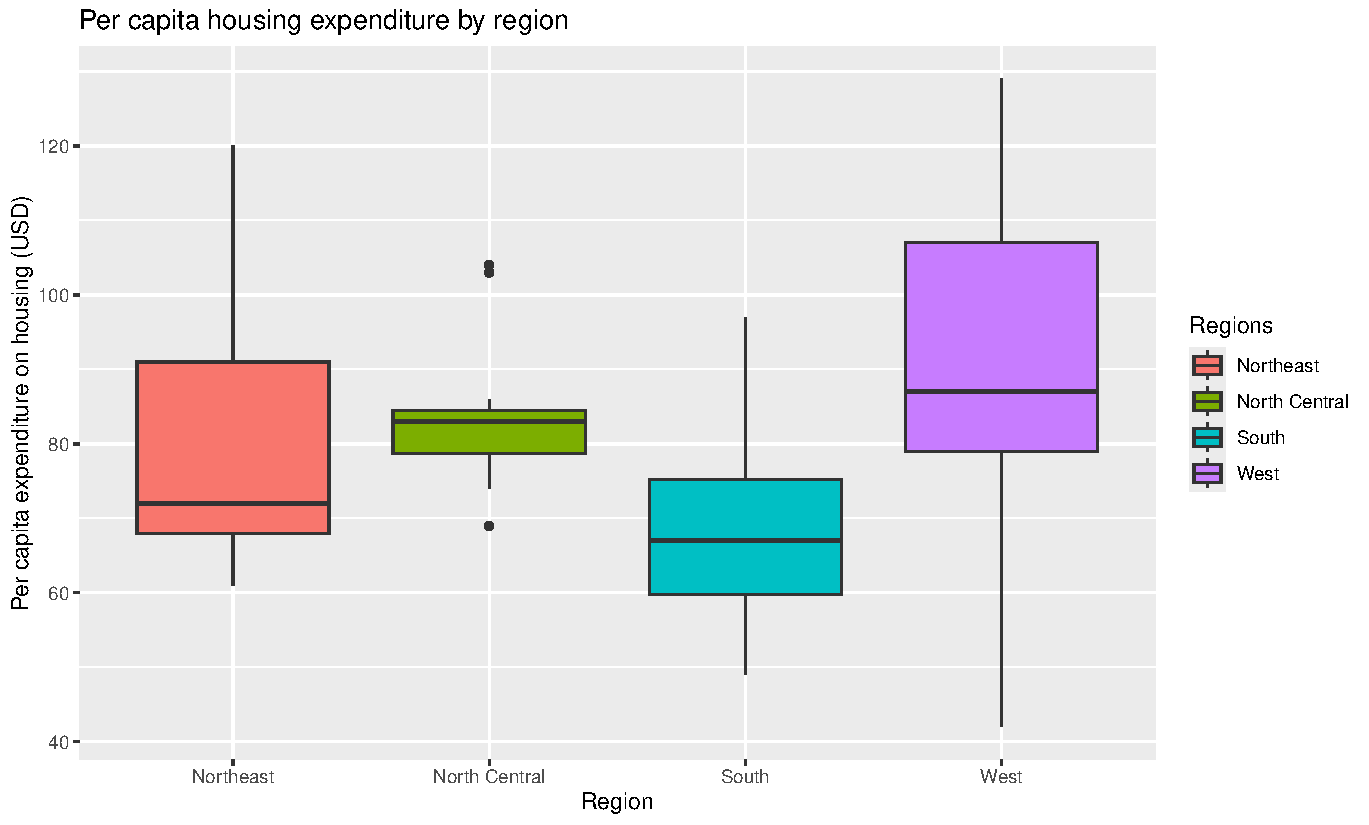
\includegraphics[scale=0.75]{housingByRegionPlot}
		
		I calculate the mean housing expenditures for each region using the following commands:
		\lstinputlisting[language=R, firstline=279, lastline=283]{PS01_answers_OS.R}
		
		The mean per capita housing expenditure in the Northeast US is 79.44 USD.
		
		The mean per capita housing expenditure in the North Central US is 83.92 USD.
		
		The mean per capita housing expenditure in the Southern US is 69.19 USD.
		
		The mean per capita housing expenditure in the Western US is 88.31 USD.
		
		\textbf{The West has the highest mean per capita housing expenditure.}
		
		\vspace{.5cm}
		\item
		Please plot the relationship between \emph{Y} and \emph{X1}? Describe this graph and the relationship. Reproduce the above graph including one more variable \emph{Region} and display different regions with different types of symbols and colors.
		
		\textbf{1. Plotting housing assistance expenditure against per capita income}
		
		I create a simple linear regression model of Y on X1 and calculate the slope, intercept, and R-squared:
		\lstinputlisting[language=R, firstline=292, lastline=295]{PS01_answers_OS.R}
		
		I then create the below scatterplot of Y on X1 using this code:
		\lstinputlisting[language=R, firstline=300, lastline=310]{PS01_answers_OS.R}
		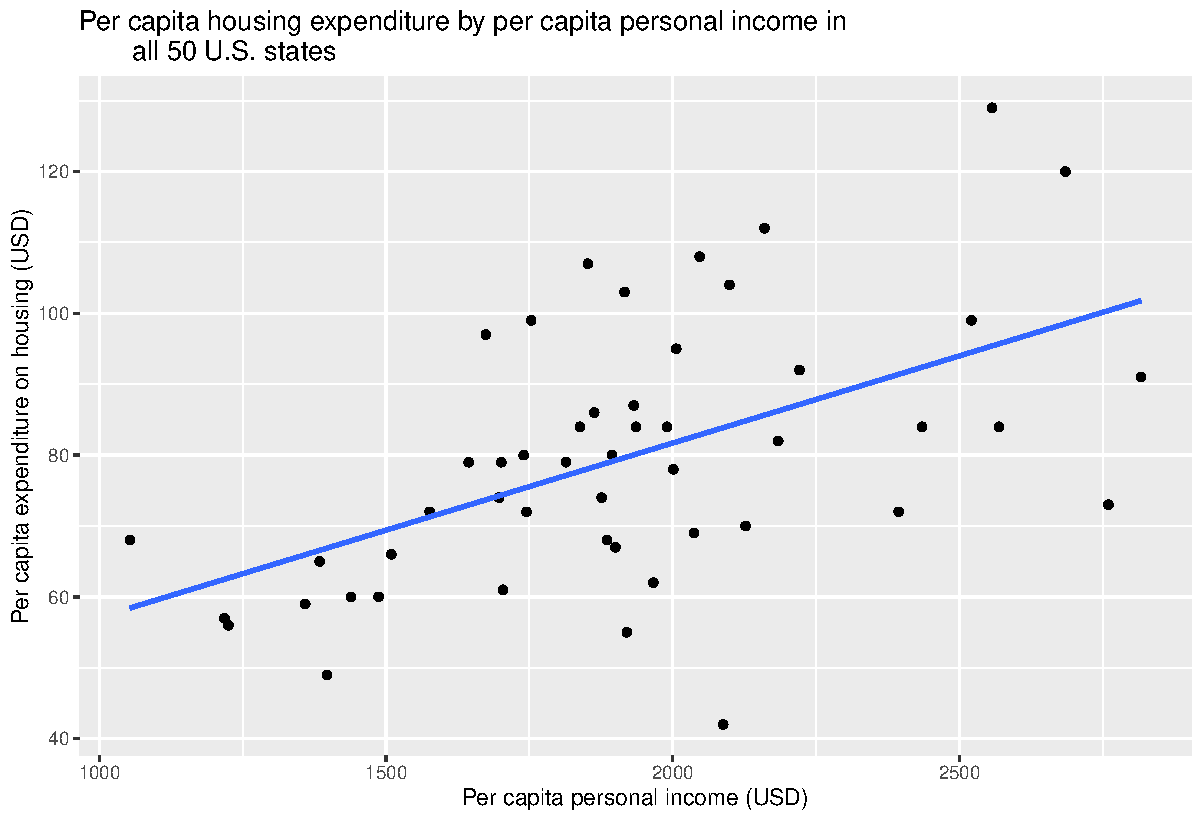
\includegraphics[scale=0.7]{housingByIncomePlot}\\
		
		This scatterplot shows a weak, positive association between per capita personal income and per capita expenditure on housing assistance. There do not appear to be any outliers in the data. The multiple R-squared value is  0.2827; the adjusted R-squared value is  0.2678. The linear regression model is \textit{per capita housing expenditure = 0.02458(per capita personal income) + 32.546152 + $\epsilon$}.
		
		\textbf{2. Comparing all four regions in the same graph}
		
		To reproduce the above graph and add different colors, symbols, and regression lines for the different regions, I run the following code:
		\lstinputlisting[language=R, firstline=322, lastline=332]{PS01_answers_OS.R}
		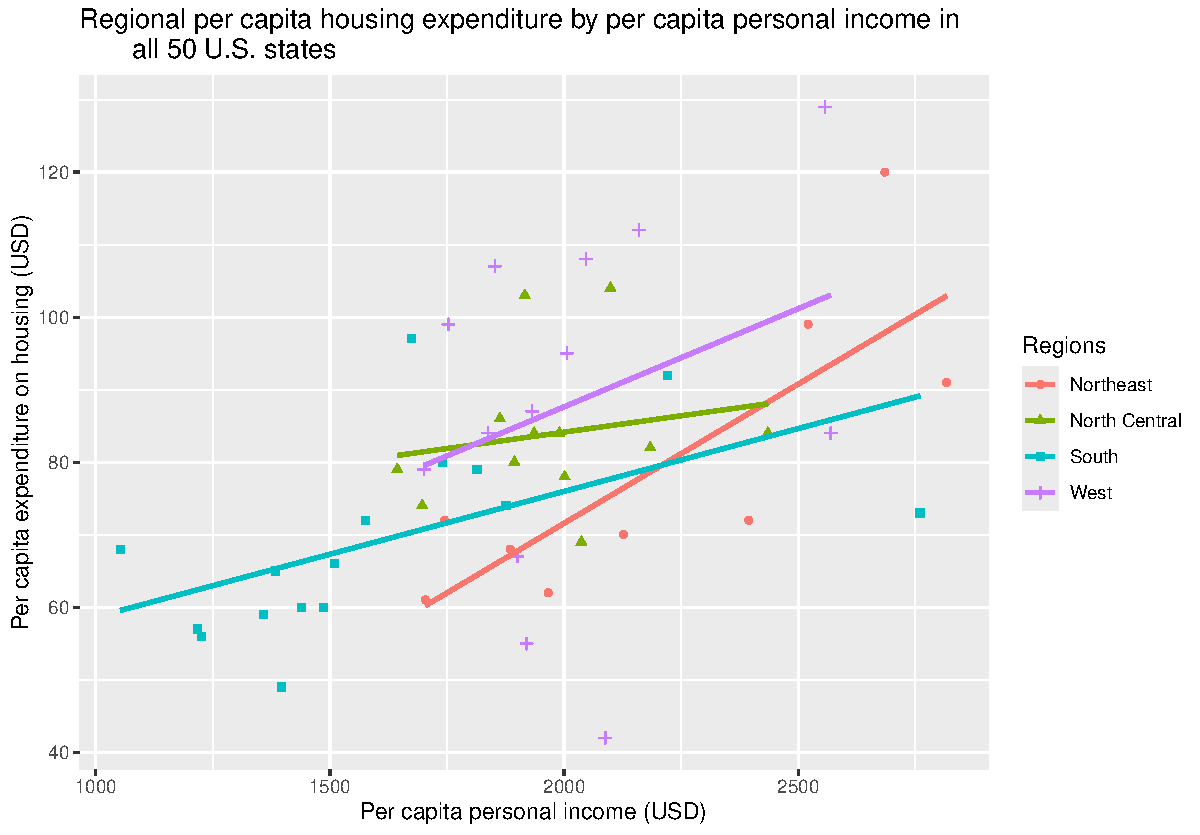
\includegraphics[scale=0.85]{regionalHousingByIncomePlot}\\
		
		Across all four regions, there appears to be a weak, positive association between per capita personal income and per capita expenditure on housing assistance. The West has the most variation in the data, perhaps due to the region's large size and inclusion of both largely rural, poorer states, e.g. Idaho, and affluent states with major urban centers, e.g. California. 
		
	\end{itemize}
	
	
\end{document}
